\documentclass[a4paper]{iacas}

\usepackage{cite}
\usepackage{hyperref}% embedding hyperlinks [must be loaded after dropping]
\usepackage{amsmath,amsthm,amssymb,amsfonts,latexsym,mathrsfs,wasysym}
\usepackage{marvosym}
\usepackage{subcaption}
\usepackage{soul,color}
\usepackage{threeparttable}% tables with footnotes
\usepackage{dcolumn}% decimal-aligned tabular math columns
\usepackage{float}
\usepackage{graphicx}
\usepackage{accents}
\usepackage{tikz}
\usepackage{lastpage}
\usepackage{fancyhdr}
\usepackage{color}
\usepackage{cancel}
\usepackage{setspace}
\usepackage{enumitem}
\usepackage{pdfpages}
\usepackage{algorithm}
\usepackage{algorithmic}


%\doublespacing
% or:
\onehalfspacing
%\usepackage[T1]{fontenc}
%\usepackage{bigfoot} % to allow verbatim in footnote
\usepackage[framed,numbered]{matlab-prettifier}
\pagestyle{plain}
%\usepackage[hebrew,english]{babel}
\usetikzlibrary{shapes.geometric, arrows, calc}

\newcolumntype{d}{D{.}{.}{-1}}
\graphicspath{{figures/}}

% define some commands to maintain consistency
\newcommand{\pkg}[1]{\texttt{#1}}
\newcommand{\cls}[1]{\textsf{#1}}
\newcommand{\file}[1]{\texttt{#1}}
\newcommand{\sgn}[1]{\operatorname{sgn}\left(#1\right)}
\newcommand{\sat}[1]{\operatorname{sat}\left(#1\right)}
\newcommand{\rrule}[1]{\rule[#1]{0pt}{0pt}}
\newcommand{\fracds}[2]{\frac{\displaystyle #1\rrule{-0.2em}}{\displaystyle #2\rrule{1em}}}
\newcommand{\figref}[1]{Fig.~\ref{#1}}
\newcommand{\ubar}[1]{\underaccent{\bar}{#1}}
\newcommand{\norm}[1]{\lvert \lvert \vec #1 \rvert \rvert}

%diffeomorphism

\begin{document}
%
%\begin{center}
% \large Image processing - 046200
% \end{center}
%\begin{center}
%\large\textbf{Homework \#4}
% \end{center}
%
%
%\begin{tabular}{l}
%\\
%{\bf\textit{Alexander Shender 328626114}} \\
%{\bf\textit{Sahar Carmel 305554453}} \\
%Technion - Israel Institute of Technology
%\end{tabular}
%
%
%\newpage
\section{Question 4.}
\subsection{}
included in the code

\subsection{}
included in the code.


\subsection{}
The algorithm did not succeed to successfully identify and match the template. The algorithm failed in the cases where the occlusion was present, or the object was rotated by a certain value. 
\newline
Example for the successful detection:

\vskip 0.1in
\begin{minipage}{0.5\textwidth}
\centering
	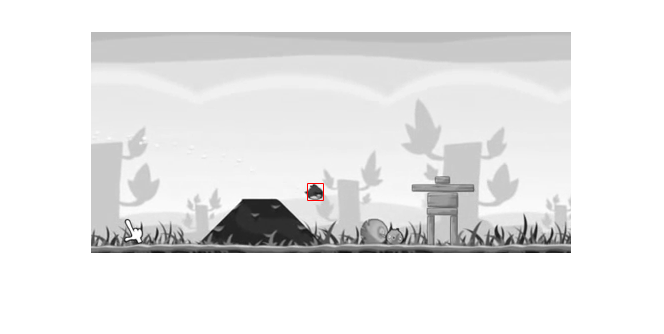
\includegraphics[scale=0.8]{output/q4/algo_1/successful.png}
\end{minipage}
\vskip 0.1in

Not successful detections:

\vskip 0.1in
\begin{minipage}{0.5\textwidth}
\centering
	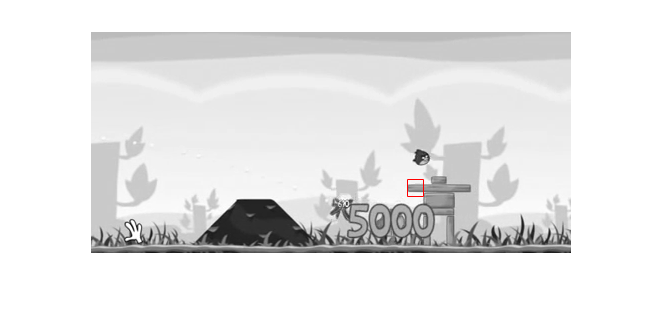
\includegraphics[scale=0.8]{output/q4/algo_1/13.png}
	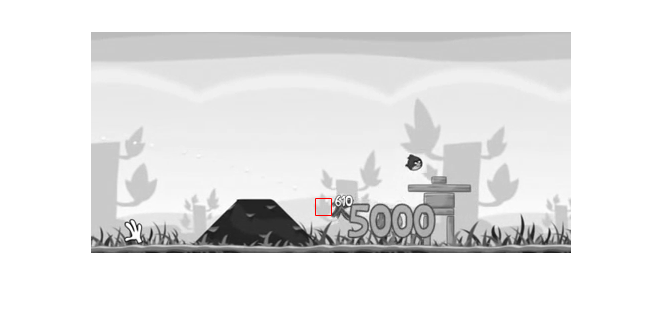
\includegraphics[scale=0.8]{output/q4/algo_1/18.png}
	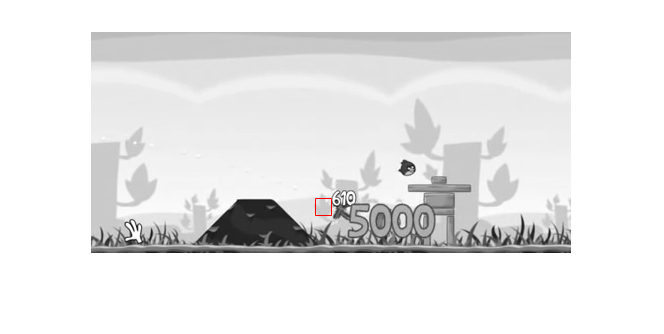
\includegraphics[scale=0.8]{output/q4/algo_1/19.png}
	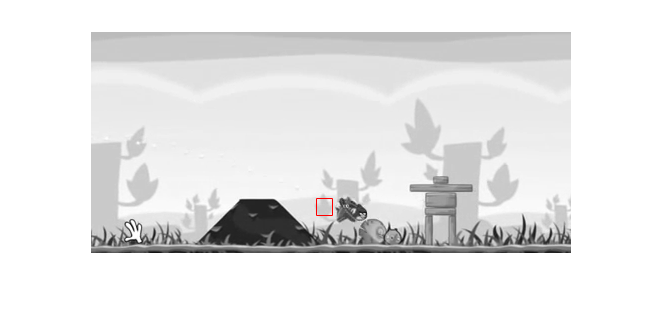
\includegraphics[scale=0.8]{output/q4/algo_1/20.png}
\end{minipage}
\vskip 0.1in

The following figure demonstrates the Maximum correlation value that was found for each of the correlations. Not surprisingly, the cases where the correlation is low, the prediction was not correct
\vskip 0.1in
\begin{minipage}{0.5\textwidth}
\centering
	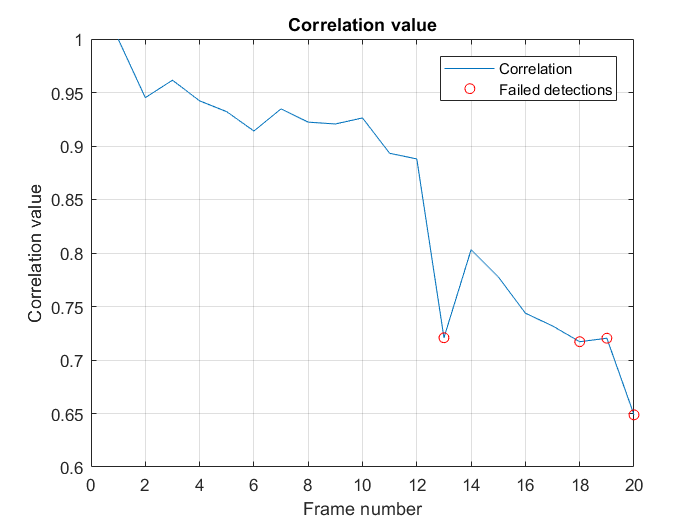
\includegraphics[scale=0.8]{output/q4/algo_1/corr_graph.png}
\end{minipage}
\vskip 0.1in

\subsection{}
There were 2 fixes to the algorithm, to deal with both of the reasons for failure. 
\begin{enumerate}
\item First, the loop was created which goes over different angles from $-\pi/2$ to $\pi/2$. This has solved the problem for the object at an angle. But still the problem of occlusion exists
The following graph shows the improvement in correlation for the last 3 frames where the detection was wrong.
\vskip 0.1in
\begin{minipage}{0.5\textwidth}
\centering
	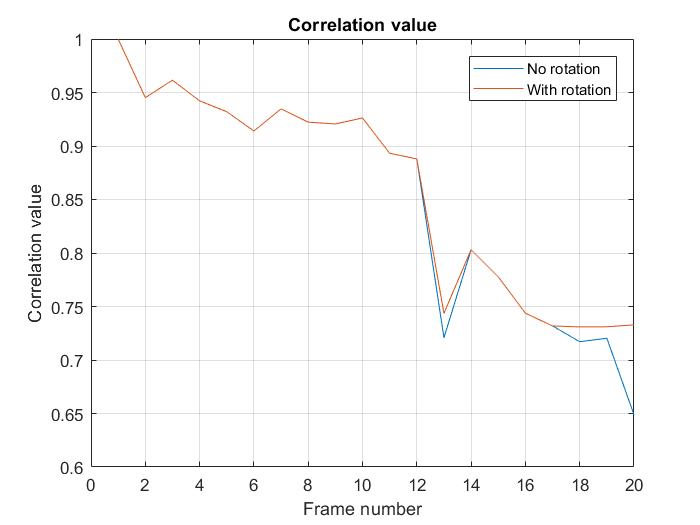
\includegraphics[scale=0.8]{output/q4/algo_2/corr.png}
\end{minipage}
\vskip 0.1in

\item To solve the problem of the occlusion, we have divided the template into 2 parts. The left part and the right part. The initial plan was to calculate the correlation for both of them, and if the found coordinates were not close enough - we take the coordinates of the template with the highest correlation value. (This case means than the second template must have been occluded and gave a low correlation value with some other object). But the reality did not go as planned, and this 'fusion' model did not succeed. What did succeed is just taking 1 part of the template, the right part (which is not occluded on the frame 13), and then all the cases detected the bird successfully. Below is the image of the Correlation values for 3 algorithms. We can see than on Frame 13, where the bird has been occluded, the correlation value was raised. (But the correlation values on the graph are normalized, so we cannot compare different algorithm correlations values).

\vskip 0.1in
\begin{minipage}{0.5\textwidth}
\centering
	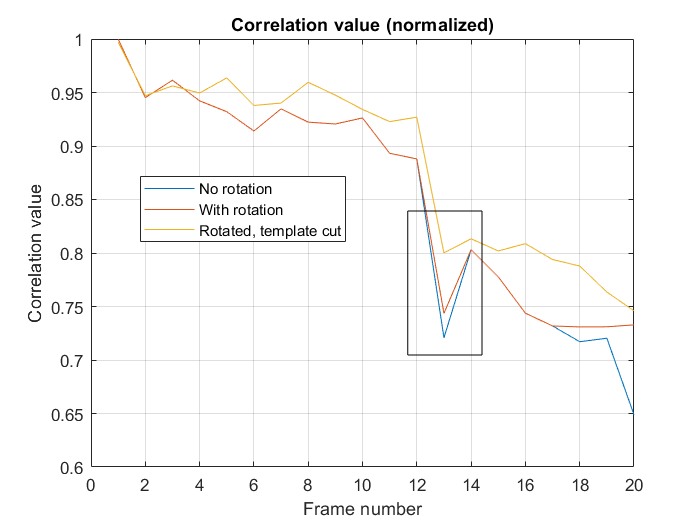
\includegraphics[scale=0.8]{output/q4/algo_3/algo_3_13_frame.png}
\end{minipage}
\vskip 0.1in

\end{enumerate}


The following images show the frames, which have previously failed, being successful again.

\vskip 0.1in
\begin{minipage}{0.5\textwidth}
\centering
	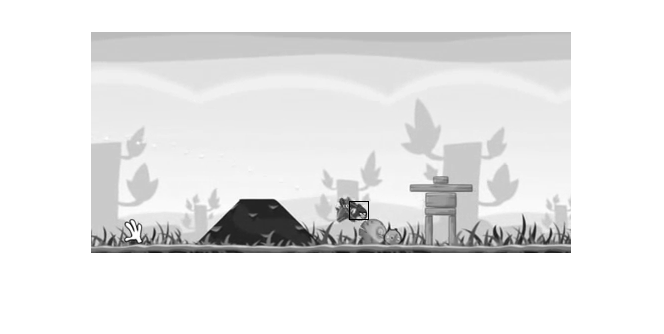
\includegraphics[scale=0.8]{output/q4/algo_3/13.png}
	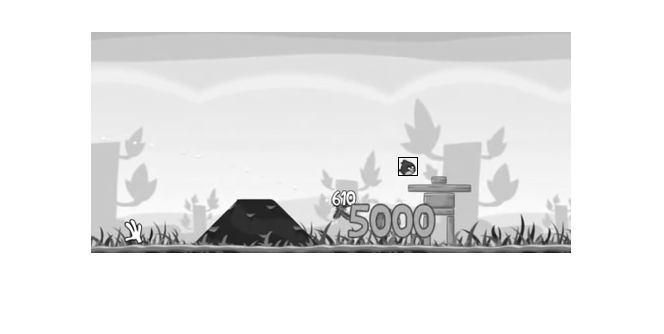
\includegraphics[scale=0.8]{output/q4/algo_3/18.png}
	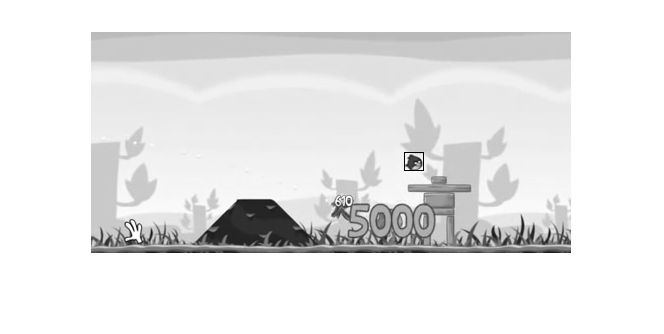
\includegraphics[scale=0.8]{output/q4/algo_3/19.png}
	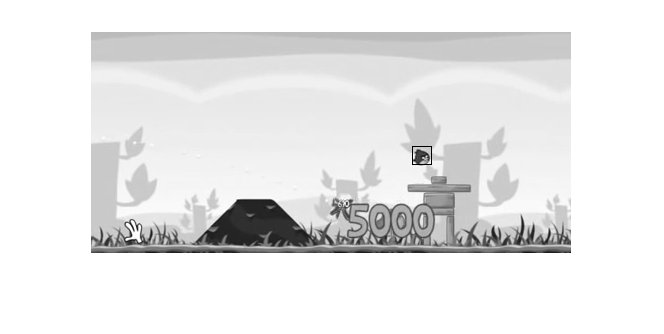
\includegraphics[scale=0.8]{output/q4/algo_3/20.png}
\end{minipage}
\vskip 0.1in



\newpage
\section{Question 5.}
\subsection{}
The circle has been built. The fuction which creates a noisy image was created as well. The following images show the circle built.


\vskip 0.1in
\begin{minipage}{0.5\textwidth}
\centering
	
\includegraphics[scale=0.8]{output/q5/circle.png}
\end{minipage}
\vskip 0.1in

\subsection{}
The function exists in the MATLAB code.

\subsection{}
By operating the L2 denoise algorithm with the prescribed parameters we obtain the following $Err_{1}$ and $Err_{2}$ results:
\vskip 0.1in
\begin{minipage}{0.5\textwidth}
\centering
	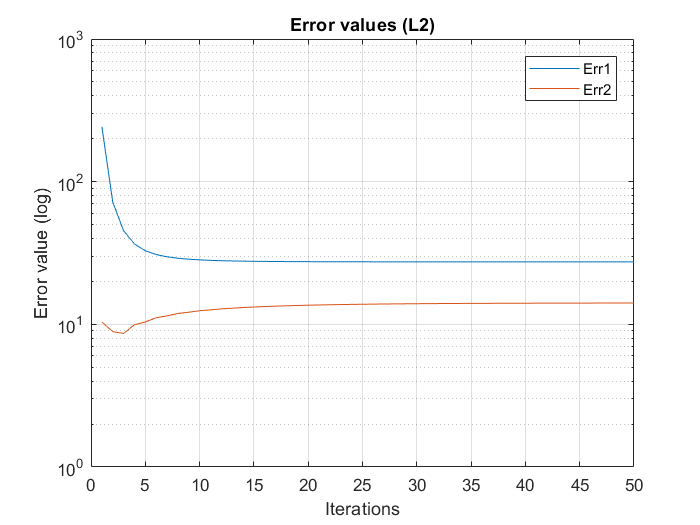
\includegraphics[scale=0.8]{output/q5/L2_err.png}
\end{minipage}
\vskip 0.1in
By printing the image every 10 iterations we obtain:
\vskip 0.1in
\begin{minipage}{0.5\textwidth}
\centering
	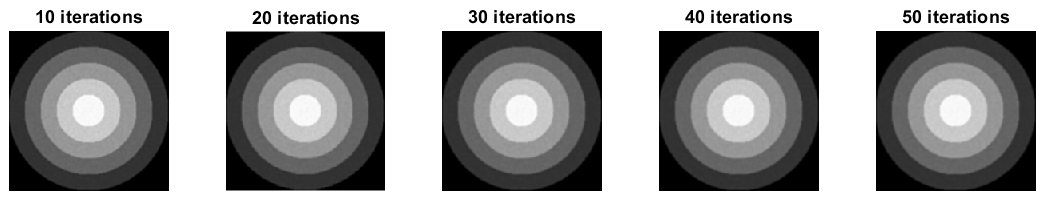
\includegraphics[scale=0.6]{output/q5/L2_iter.png}
\end{minipage}
\vskip 0.1in

It is definitely hard to distinguish the image with the least noise from those images. So we take the minimum value from the $Err_{2}$ graph, which shows the difference of the de-noised image from the original image. We obtain this value at the iteration=3. Displaying the best image from the best iteration:

\begin{minipage}{0.5\textwidth}
\centering
	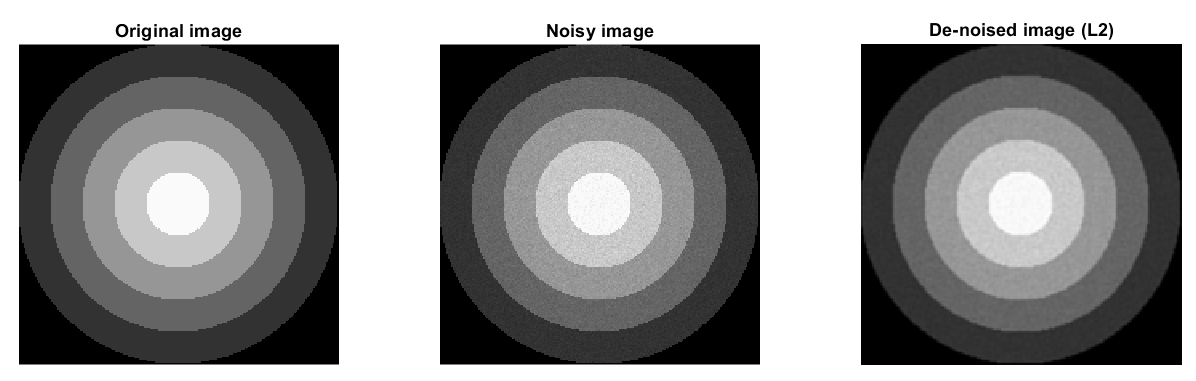
\includegraphics[scale=0.5]{output/q5/L2_denoise.png}
\end{minipage}
\vskip 0.1in

We can observe than some denoising did take place indeed, the image became smoother. Also the edges got smoother, which should be fixed with the TV prior, which we see in the next subsection.

\subsection{}
The parameters were set as prescribed, the results obtained are the following. For the error values:

\vskip 0.1in
\begin{minipage}{0.5\textwidth}
\centering
	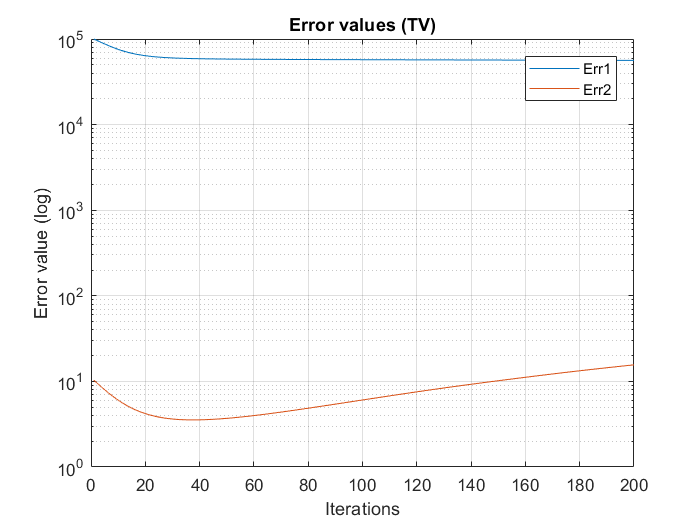
\includegraphics[scale=0.8]{output/q5/TV_err.png}
\end{minipage}
\vskip 0.1in
By printing the image every 50 iterations we obtain:
\vskip 0.1in
\begin{minipage}{0.5\textwidth}
\centering
	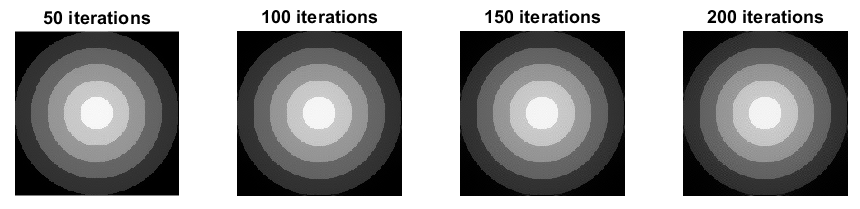
\includegraphics[scale=0.6]{output/q5/TV_iter.png}
\end{minipage}
\vskip 0.1in

Similarly, it is hard to choose the best image by looking at them. So we choose at the iteration with the smallest $Err_{2}$ value. This happens approximately at iteration 30. Displaying this best result:

\vskip 0.1in
\begin{minipage}{0.5\textwidth}
\centering
	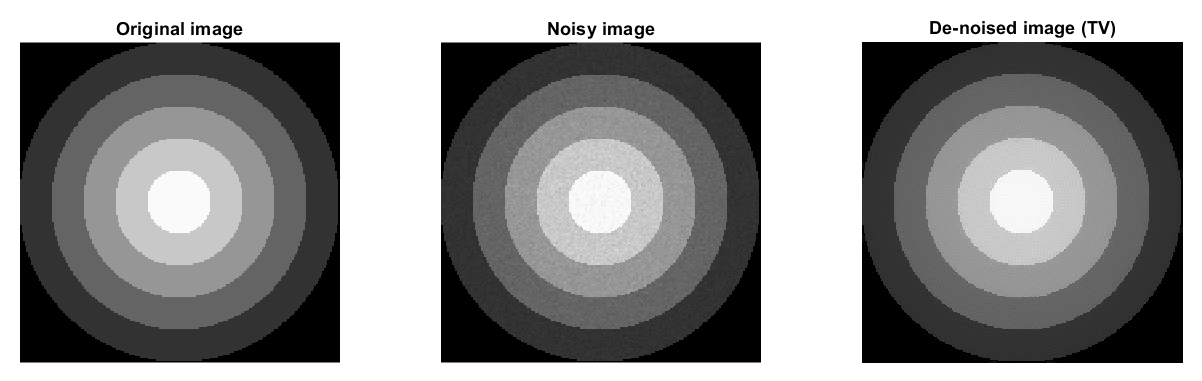
\includegraphics[scale=0.5]{output/q5/TV_denoise.png}
\end{minipage}
\vskip 0.1in

We can see the improvement, also by looking at the minimal $Err_{2}$ value for both methods. More on this in next subsection.

\subsection{}
Let's first compare both denoises:
\vskip 0.1in
\begin{minipage}{0.5\textwidth}
\centering
	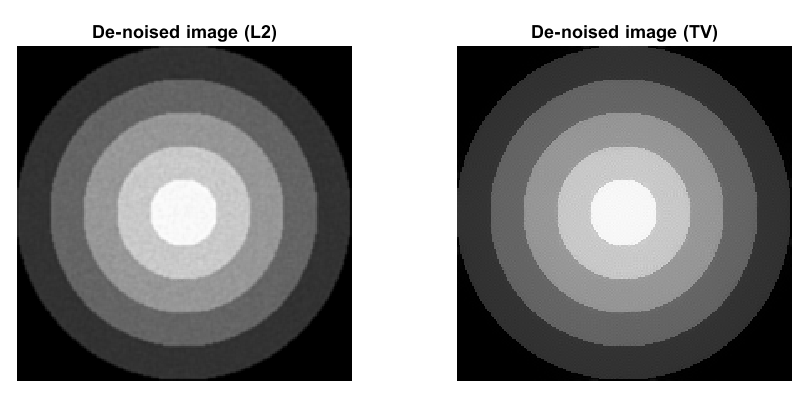
\includegraphics[scale=0.7]{output/q5/L2_TV.png}
\end{minipage}
\vskip 0.1in

Several things can be said:

\begin{enumerate}
\item The denoise process with the TV prior performs better than with the L2 prior
\item TV tends to preserve the edges!
\item L2 tends to blur both noise, and edges, without distinguising between the two
\end{enumerate}


\subsection{}
The image taken is presented below. The same noise was added to it. Below are presented 3 images:

\begin{enumerate}
\item The original image
\vskip 0.1in
\begin{minipage}{0.5\textwidth}
\centering
	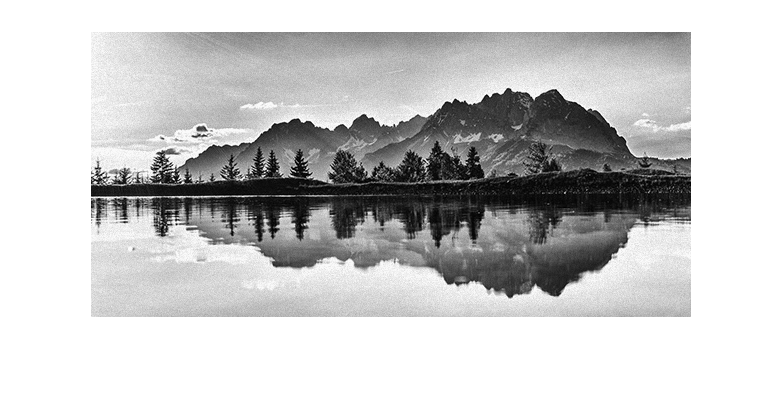
\includegraphics[scale=0.7]{output/q5/original_image.png}
\end{minipage}
\vskip 0.1in


\item The de-noise by L2 prior

\vskip 0.1in
\begin{minipage}{0.5\textwidth}
\centering
	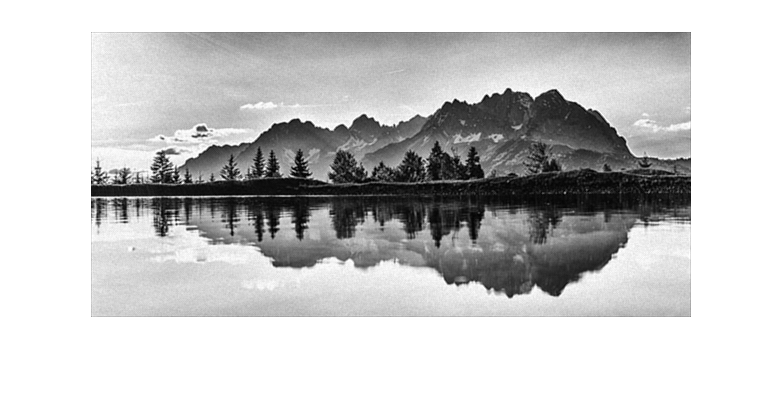
\includegraphics[scale=0.7]{output/q5/image_L2_denoise.png}
\end{minipage}
\vskip 0.1in

\item The de-noise by TV prior

\vskip 0.1in
\begin{minipage}{0.5\textwidth}
\centering
	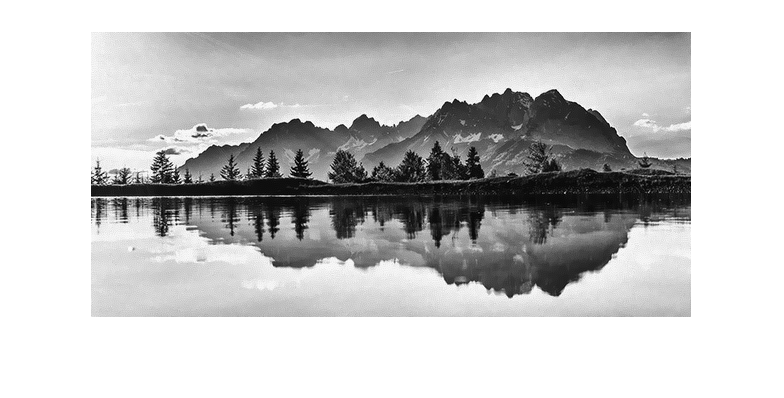
\includegraphics[scale=0.7]{output/q5/image_TV_denoise.png}
\end{minipage}
\vskip 0.1in

We can indeed see that the de-noise using the TV prior is much more successful and gives better results
\end{enumerate}




\end{document}



















